\documentclass{standalone}
\usepackage{tikz}
\usetikzlibrary{patterns, positioning}

\begin{document}
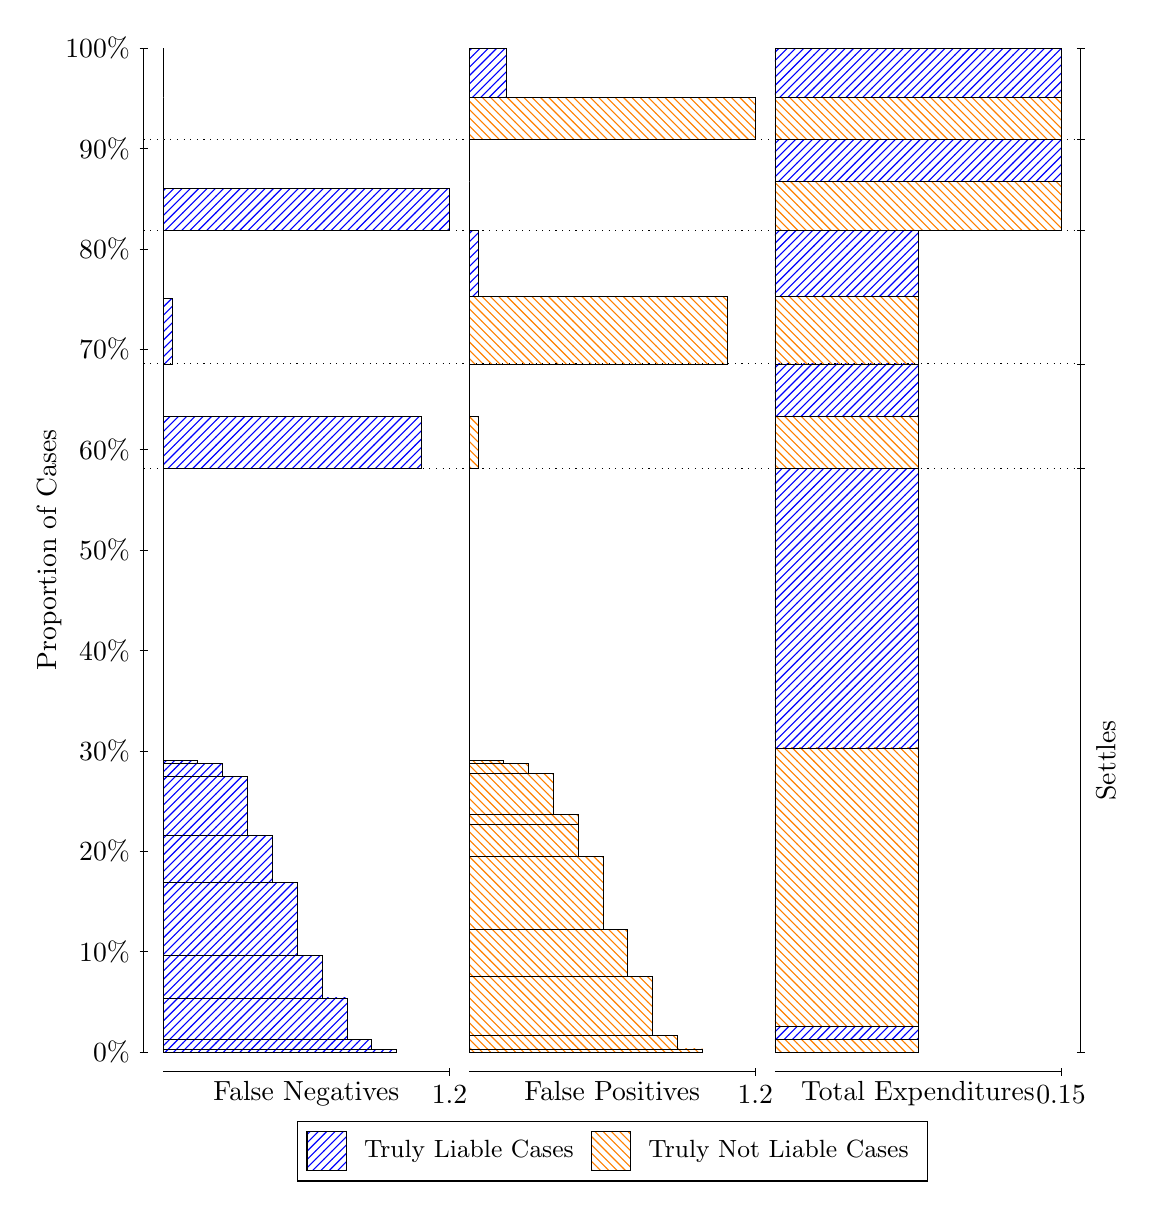
\begin{tikzpicture}
\draw[black, very thin] (1.5,1.75) -- (1.5,14.5);
\node[rotate=90, anchor=center] at (0.3, 8.125) {Proportion of Cases};
\draw[black, very thin] (1.45,1.75) -- (1.55,1.75);
\node[anchor=east] at (1.45, 1.75) {0\%};
\draw[black, very thin] (1.45,3.025) -- (1.55,3.025);
\node[anchor=east] at (1.45, 3.025) {10\%};
\draw[black, very thin] (1.45,4.3) -- (1.55,4.3);
\node[anchor=east] at (1.45, 4.3) {20\%};
\draw[black, very thin] (1.45,5.575) -- (1.55,5.575);
\node[anchor=east] at (1.45, 5.575) {30\%};
\draw[black, very thin] (1.45,6.85) -- (1.55,6.85);
\node[anchor=east] at (1.45, 6.85) {40\%};
\draw[black, very thin] (1.45,8.125) -- (1.55,8.125);
\node[anchor=east] at (1.45, 8.125) {50\%};
\draw[black, very thin] (1.45,9.4) -- (1.55,9.4);
\node[anchor=east] at (1.45, 9.4) {60\%};
\draw[black, very thin] (1.45,10.675) -- (1.55,10.675);
\node[anchor=east] at (1.45, 10.675) {70\%};
\draw[black, very thin] (1.45,11.95) -- (1.55,11.95);
\node[anchor=east] at (1.45, 11.95) {80\%};
\draw[black, very thin] (1.45,13.225) -- (1.55,13.225);
\node[anchor=east] at (1.45, 13.225) {90\%};
\draw[black, very thin] (1.45,14.5) -- (1.55,14.5);
\node[anchor=east] at (1.45, 14.5) {100\%};

\draw[black, very thin] (13.4,1.75) -- (13.4,14.5);
\draw[black, very thin] (13.35,1.75) -- (13.45,1.75);
\node[anchor=west] at (13.35, 1.75) {};
\draw[black, very thin] (13.35,9.1576) -- (13.45,9.1576);
\node[anchor=west] at (13.35, 9.1576) {};
\draw[black, very thin] (13.35,10.488) -- (13.45,10.488);
\node[anchor=west] at (13.35, 10.488) {};
\draw[black, very thin] (13.35,12.182) -- (13.45,12.182);
\node[anchor=west] at (13.35, 12.182) {};
\draw[black, very thin] (13.35,13.34) -- (13.45,13.34);
\node[anchor=west] at (13.35, 13.34) {};
\draw[black, very thin] (13.35,14.5) -- (13.45,14.5);
\node[anchor=west] at (13.35, 14.5) {};

\draw[black, very thin, pattern color=blue, pattern=north east lines] (1.75,1.75) rectangle (4.712,1.7861);
\draw[black, very thin, pattern color=blue, pattern=north east lines] (1.75,1.7861) rectangle (4.396,1.9087);
\draw[black, very thin, pattern color=blue, pattern=north east lines] (1.75,1.9087) rectangle (4.0801,2.4372);
\draw[black, very thin, pattern color=blue, pattern=north east lines] (1.75,2.4372) rectangle (3.7641,2.9732);
\draw[black, very thin, pattern color=blue, pattern=north east lines] (1.75,2.9732) rectangle (3.4482,3.9045);
\draw[black, very thin, pattern color=blue, pattern=north east lines] (1.75,3.9045) rectangle (3.1322,4.4979);
\draw[black, very thin, pattern color=blue, pattern=north east lines] (1.75,4.4979) rectangle (2.8163,5.2466);
\draw[black, very thin, pattern color=blue, pattern=north east lines] (1.75,5.2466) rectangle (2.5004,5.4142);
\draw[black, very thin, pattern color=blue, pattern=north east lines] (1.75,5.4142) rectangle (2.1844,5.4554);
\draw[black, very thin, pattern color=orange, pattern=north west lines] (1.75,5.4554) rectangle (1.75,9.1576);
\draw[black, very thin, pattern color=blue, pattern=north east lines] (1.75,9.1576) rectangle (5.0279,9.8246);
\draw[black, very thin, pattern color=orange, pattern=north west lines] (1.75,9.8246) rectangle (1.75,10.488);
\draw[black, very thin, pattern color=blue, pattern=north east lines] (1.75,10.488) rectangle (1.8685,11.324);
\draw[black, very thin, pattern color=orange, pattern=north west lines] (1.75,11.324) rectangle (1.75,12.182);
\draw[black, very thin, pattern color=blue, pattern=north east lines] (1.75,12.182) rectangle (5.3833,12.717);
\draw[black, very thin, pattern color=orange, pattern=north west lines] (1.75,12.717) rectangle (1.75,13.34);
\draw[black, very thin, pattern color=orange, pattern=north west lines] (1.75,13.34) rectangle (1.75,13.869);
\draw[black, very thin, pattern color=blue, pattern=north east lines] (1.75,13.869) rectangle (1.75,14.5);
\draw[black, very thin, pattern color=orange, pattern=north west lines] (5.6333,1.75) rectangle (8.5953,1.7892);
\draw[black, very thin, pattern color=orange, pattern=north west lines] (5.6333,1.7892) rectangle (8.2793,1.9566);
\draw[black, very thin, pattern color=orange, pattern=north west lines] (5.6333,1.9566) rectangle (7.9634,2.7127);
\draw[black, very thin, pattern color=orange, pattern=north west lines] (5.6333,2.7127) rectangle (7.6475,3.3048);
\draw[black, very thin, pattern color=orange, pattern=north west lines] (5.6333,3.3048) rectangle (7.3315,4.231);
\draw[black, very thin, pattern color=orange, pattern=north west lines] (5.6333,4.231) rectangle (7.0156,4.6379);
\draw[black, very thin, pattern color=orange, pattern=north west lines] (5.6333,4.6379) rectangle (7.0156,4.763);
\draw[black, very thin, pattern color=orange, pattern=north west lines] (5.6333,4.763) rectangle (6.6996,5.2907);
\draw[black, very thin, pattern color=orange, pattern=north west lines] (5.6333,5.2907) rectangle (6.3837,5.4155);
\draw[black, very thin, pattern color=orange, pattern=north west lines] (5.6333,5.4155) rectangle (6.0678,5.4523);
\draw[black, very thin, pattern color=blue, pattern=north east lines] (5.6333,5.4523) rectangle (5.6333,9.1576);
\draw[black, very thin, pattern color=orange, pattern=north west lines] (5.6333,9.1576) rectangle (5.7518,9.8206);
\draw[black, very thin, pattern color=blue, pattern=north east lines] (5.6333,9.8206) rectangle (5.6333,10.488);
\draw[black, very thin, pattern color=orange, pattern=north west lines] (5.6333,10.488) rectangle (8.9112,11.345);
\draw[black, very thin, pattern color=blue, pattern=north east lines] (5.6333,11.345) rectangle (5.7518,12.182);
\draw[black, very thin, pattern color=orange, pattern=north west lines] (5.6333,12.182) rectangle (5.6333,12.805);
\draw[black, very thin, pattern color=blue, pattern=north east lines] (5.6333,12.805) rectangle (5.6333,13.34);
\draw[black, very thin, pattern color=orange, pattern=north west lines] (5.6333,13.34) rectangle (9.2667,13.869);
\draw[black, very thin, pattern color=blue, pattern=north east lines] (5.6333,13.869) rectangle (6.1072,14.5);
\draw[black, very thin, pattern color=orange, pattern=north west lines] (9.5167,1.75) rectangle (11.333,1.9116);
\draw[black, very thin, pattern color=blue, pattern=north east lines] (9.5167,1.9116) rectangle (11.333,2.0703);
\draw[black, very thin, pattern color=orange, pattern=north west lines] (9.5167,2.0703) rectangle (11.333,5.611);
\draw[black, very thin, pattern color=blue, pattern=north east lines] (9.5167,5.611) rectangle (11.333,9.1576);
\draw[black, very thin, pattern color=orange, pattern=north west lines] (9.5167,9.1576) rectangle (11.333,9.8206);
\draw[black, very thin, pattern color=blue, pattern=north east lines] (9.5167,9.8206) rectangle (11.333,10.488);
\draw[black, very thin, pattern color=orange, pattern=north west lines] (9.5167,10.488) rectangle (11.333,11.345);
\draw[black, very thin, pattern color=blue, pattern=north east lines] (9.5167,11.345) rectangle (11.333,12.182);
\draw[black, very thin, pattern color=orange, pattern=north west lines] (9.5167,12.182) rectangle (13.15,12.805);
\draw[black, very thin, pattern color=blue, pattern=north east lines] (9.5167,12.805) rectangle (13.15,13.34);
\draw[black, very thin, pattern color=orange, pattern=north west lines] (9.5167,13.34) rectangle (13.15,13.869);
\draw[black, very thin, pattern color=blue, pattern=north east lines] (9.5167,13.869) rectangle (13.15,14.5);
\draw[black, dotted] (1.5,9.1576) -- (13.4,9.1576);
\draw[black, dotted] (1.5,10.488) -- (13.4,10.488);
\draw[black, dotted] (1.5,12.182) -- (13.4,12.182);
\draw[black, dotted] (1.5,13.34) -- (13.4,13.34);
\draw[black, very thin] (1.75,1.5) -- (5.3833,1.5);
\node[anchor=north] at (3.5667, 1.5) {False Negatives};
\draw[black, very thin] (5.3833,1.45) -- (5.3833,1.55);
\node[anchor=north] at (5.3833, 1.45) {1.2};

\draw[black, very thin] (5.6333,1.5) -- (9.2667,1.5);
\node[anchor=north] at (7.45, 1.5) {False Positives};
\draw[black, very thin] (9.2667,1.45) -- (9.2667,1.55);
\node[anchor=north] at (9.2667, 1.45) {1.2};

\draw[black, very thin] (9.5167,1.5) -- (13.15,1.5);
\node[anchor=north] at (11.333, 1.5) {Total Expenditures};
\draw[black, very thin] (13.15,1.45) -- (13.15,1.55);
\node[anchor=north] at (13.15, 1.45) {0.15};

\node[black, centered, rotate=90] at (13.72, 5.4538) {Settles};





\draw (7.449999999999999,1.5) node[draw=none] (baseCoordinate) {};
\begin{scope}[align=center]
        \matrix[scale=0.5, draw=black, below=0.5cm of baseCoordinate, nodes={draw}, column sep=0.1cm]{
            \node[rectangle, draw, minimum width=0.5cm, minimum height=0.5cm, pattern=north east lines, pattern color=blue] {}; &
            \node[draw=none, font=\small] (B) {Truly Liable Cases}; &
            \node[rectangle, draw, minimum width=0.5cm, minimum height=0.5cm, pattern=north west lines, pattern color=orange] {}; &
            \node[draw=none, font=\small] (B) {Truly Not Liable Cases}; \\
            };
\end{scope}

\end{tikzpicture}
\end{document}